\section{Introduction}

% What is the problem?
Today's client-server based file system metadata services have scalability
problems. It takes a lot of resources to service POSIX metadata requests so
applications perform better with dedicated metadata
servers~\cite{sevilla:sc15-mantle, ren:sc2014-indexfs}. Unfortunately,
provisioning a metadata server for every client is expensive and complicated.

% How does this fit in current landscape?
Current hardware evolution and the rise of software-defined storage storage,
which uses techniqes like erasure coding, replication, and partitioning, have
ushered in a new era of HPC computing; architectures are transitioning from
complex storage stacks with burst buffer, file system, object store, and tape
tiers to a two layer stack with just a burst buffer and object
store~\cite{bent:login16-hpc-trends}. This trend exacerbates the metadata
scalability problem 

% What is HPC doing?
To address this trend, HPC research has advocated client side processing and an
emphasis on serverless metadata services.  The techniques propose new metadata
management techniques that reduce synchronization and serialization overheads
by transferring these responsibilities to the client. We call this approach
``decoupling the namespace" and the semantics of consistency differ amongst
systems.  While the performance benefits are obvious for these users,
applications that rely on stronger consistency or durability guarantees must be
re-written or deployed on a different system.  

\begin{figure}[tb]
\centering
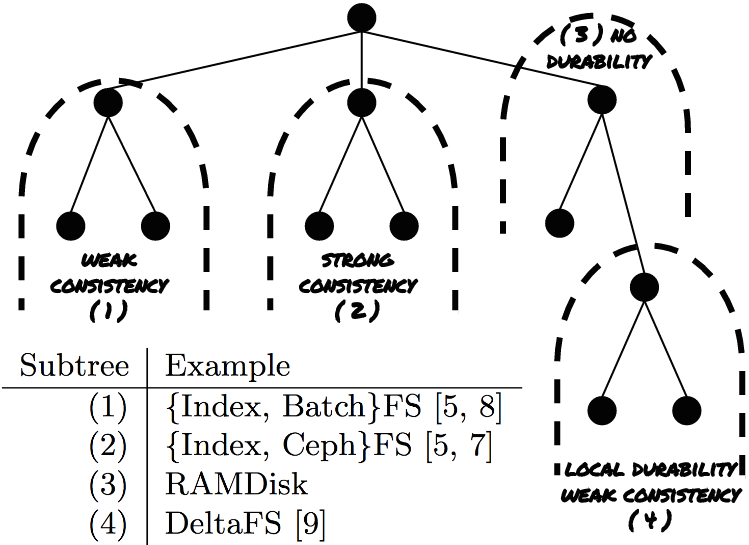
\includegraphics[width=75mm]{figures/subtree-policies.png}
\caption{Administrators can assign consistency and fault tolerance policies to
subtrees to get the benefits of some of the state-of-the-art HPC architectures.
}\label{fig:subtree-policies}
\end{figure}

% What did we do
We propose subtree policies, an interface that lets future programmers control
how the system manages different parts of the namespace.  For performance one
subtree can adopt weaker consistency semantics while another subtree can retain
the rigidity of POSIX's strong consistency. Figure~\ref{fig:subtree-policies}
shows an example setup where a single global namespace has directories for
applications designed for different, state-of-the-art HPC architectures.  We
present Cudele, a prototype programmable file system that supports different
degrees of consistency and durability by exposing mechanisms used within the
file system as a client library.  Cudele supports 3 forms of consistency
(invisible, eventual, and strong) and 3 degrees of durability (none, local, and
global) giving the administrator a wide range of policies and optimizations
that can be custom fit to an application. Our contributions: 

\begin{enumerate}

  \item a prototype that lets administrators program a range of
  consistency and durability semantics (9 permutations), allowing them to custom
  fit the storage system to the application.

  \item an API for assigning and programming policies to subtrees in the file
  system namespace.

  \item an analysis of recently proposed research systems compared against
  previously unexplored metadata designs.

\end{enumerate}

% Results
Our results confirm the assertions of ``clean-state" research systems that
decouple namespaces; specifically that the technique drastically improve
performance (104\(\times\) speed up) but we go a step further by quantifying
the costs of merging updates (7\(\times\) slow down) and maintaining durability
(\(10\times\) slow down). We also show the effect of having a metadata specific
file format in systems that are based on in-memory data structures.
Section~\ref{sec:related-work} places Cudele in the context of other related
work. Section~\ref{sec:posix-overheads} quantifies the cost of POSIX
consistency and system-defined durability and
Section~\ref{sec:methodology-decoupled-namespaces} presents the Cudele
prototype and API. Section~\ref{sec:implementation} describes Cudele's
mechanisms and shows how re-using internal subsystems results in an
implementation of less than 500 lines of code. The evaluation in
Section~\ref{sec:evaluation} quantifies the overheads and performance gains of
explored and previously unexplored metadata designs.

